\documentclass[aspectratio=169, 11pt]{beamer}

\usepackage[T1]{fontenc}
\usepackage[utf8]{inputenc}
\usepackage{helvet}
\renewcommand{\familydefault}{\sfdefault}
\usepackage{xcolor}
\usepackage{tikz}
\usetikzlibrary{arrows.meta, positioning, fit, calc, shapes.geometric}
\usepackage{booktabs}
\usepackage{microtype}

\definecolor{kblue}{HTML}{00539F}
\definecolor{kbluedark}{HTML}{003D7A}
\definecolor{kbluelight}{HTML}{E8F2FB}
\definecolor{kbluepale}{HTML}{F4F8FC}
\definecolor{kvideogray}{HTML}{C8D0D8}
\definecolor{kscreenbg}{HTML}{EEF2F7}
\definecolor{korange}{HTML}{E87722}
\definecolor{kgreen}{HTML}{2E8B57}
\definecolor{kgray}{HTML}{6C757D}
\definecolor{klightgray}{HTML}{F0F2F4}

\usetheme{default}
\setbeamercolor{background canvas}{bg=white}
\setbeamercolor{frametitle}{fg=white, bg=kblue}
\setbeamerfont{frametitle}{size=\large, series=\bfseries, family=\sffamily}
\setbeamertemplate{navigation symbols}{}
\setbeamertemplate{footline}{%
  \hfill\tiny\color{kgray}\insertframenumber\hspace{6pt}\vspace{4pt}%
}
\setbeamertemplate{frametitle}{%
  \begin{beamercolorbox}[wd=\paperwidth, ht=0.65cm, dp=0.15cm, leftskip=0.4cm]{frametitle}%
    \usebeamerfont{frametitle}\insertframetitle%
  \end{beamercolorbox}%
}

\tikzset{
  farrow/.style={-{Stealth[length=4pt, width=3pt]}, kgray, line width=0.5pt},
}

\begin{document}

{
\setbeamercolor{background canvas}{bg=kblue}
\setbeamertemplate{footline}{}
\begin{frame}
\begin{tikzpicture}[remember picture, overlay]
  \node[anchor=north west, font=\fontsize{28}{32}\selectfont\sffamily\bfseries, text=white]
    at ($(current page.north west)+(1.0,-1.2)$) {Uncanny Valley};
  \node[anchor=north west, font=\large\sffamily, text=white!75]
    at ($(current page.north west)+(1.0,-2.3)$) {Article Summaries --- Section 1};
  \draw[white!40, line width=0.5pt] ($(current page.north west)+(1.0,-3.0)$)
    -- ($(current page.north west)+(11.0,-3.0)$);
  \node[anchor=north west, font=\normalsize\sffamily, text=white!80]
    at ($(current page.north west)+(1.0,-3.4)$) {Mori 1970 \textbullet{} MacDorman \& Ishiguro 2006 \textbullet{} Ho \& MacDorman 2010 \textbullet{} McDonnell et al.\ 2012 \textbullet{} Seymour et al.\ 2021};
  \node[anchor=south west, font=\small\sffamily, text=white!60]
    at ($(current page.south west)+(1.0,0.5)$)
    {Nidanur G\"unay \quad\textbullet\quad University of Konstanz \quad\textbullet\quad 2026};
\end{tikzpicture}
\end{frame}
}

%% ═══════════════════════════════════════════════════════════════════════════
%% Mori 1970
%% ═══════════════════════════════════════════════════════════════════════════
\begin{frame}{Mori (1970) \textnormal{\normalsize --- The Uncanny Valley}}
\begin{center}
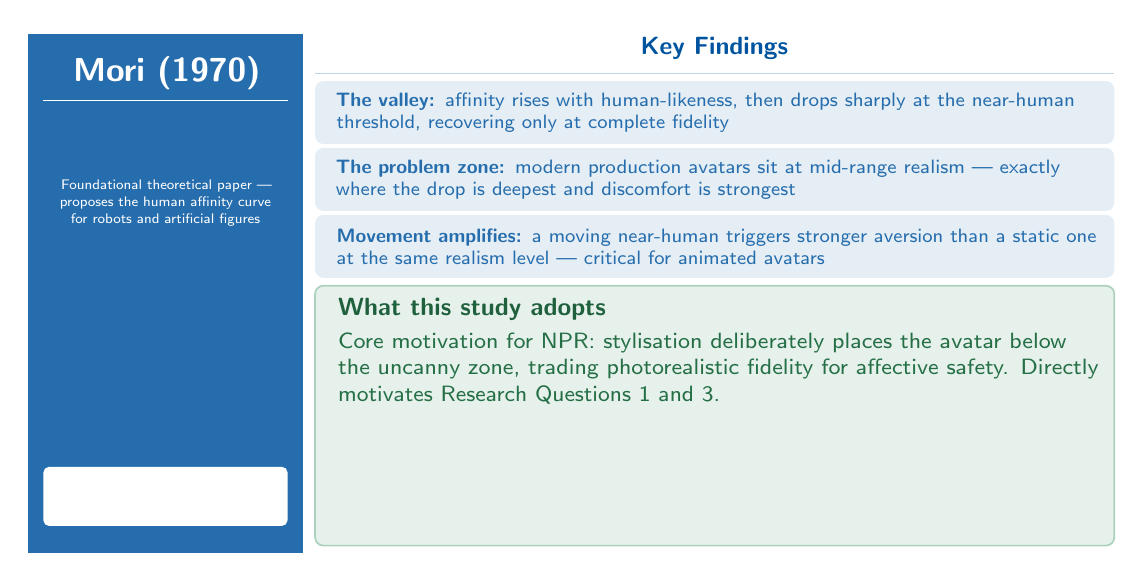
\begin{tikzpicture}[x=1cm, y=1cm]
\fill[kblue!85] (0.0,0.0) rectangle (3.5,6.6);
\node[font=\large\sffamily\bfseries, text=white, align=center, text width=3.1cm]
  at (1.75,6.10) {Mori (1970)};
\draw[white!30, line width=0.3pt] (0.2,5.75) -- (3.3,5.75);
\node[font=\tiny\sffamily, text=white!85, align=center, text width=3.0cm]
  at (1.75,4.45) {Foundational theoretical paper --- proposes the human affinity curve for robots and artificial figures};
\fill[white!20, rounded corners=2pt] (0.2,0.35) rectangle (3.3,1.10);
\node[font=\tiny\sffamily\bfseries, text=white, align=center]
  at (1.75,0.72) {Theoretical\\no experiment};
\node[font=\small\sffamily\bfseries\color{kblue}] at (8.72,6.42) {Key Findings};
\draw[kblue!25, line width=0.3pt] (3.65,6.10) -- (13.8,6.10);
\fill[kblue!10, rounded corners=3pt] (3.65,5.20) rectangle (13.8,6.00);
\node[font=\scriptsize\sffamily\color{kblue!85}, anchor=west, text width=9.65cm]
  at (3.80,5.60) {\textbf{The valley:} affinity rises with human-likeness, then drops sharply at the near-human threshold, recovering only at complete fidelity};
\fill[kblue!10, rounded corners=3pt] (3.65,4.35) rectangle (13.8,5.15);
\node[font=\scriptsize\sffamily\color{kblue!85}, anchor=west, text width=9.65cm]
  at (3.80,4.75) {\textbf{The problem zone:} modern production avatars sit at mid-range realism --- exactly where the drop is deepest and discomfort is strongest};
\fill[kblue!10, rounded corners=3pt] (3.65,3.50) rectangle (13.8,4.30);
\node[font=\scriptsize\sffamily\color{kblue!85}, anchor=west, text width=9.65cm]
  at (3.80,3.90) {\textbf{Movement amplifies:} a moving near-human triggers stronger aversion than a static one at the same realism level --- critical for animated avatars};
\fill[kgreen!12, draw=kgreen!40, rounded corners=3pt, line width=0.6pt]
  (3.65,0.1) rectangle (13.8,3.40);
\node[font=\small\sffamily\bfseries\color{kgreen!70!black}, anchor=west]
  at (3.82,3.1) {What this study adopts};
\node[font=\footnotesize\sffamily\color{kgreen!80!black}, anchor=north west, text width=9.65cm]
  at (3.82,2.92) {Core motivation for NPR: stylisation deliberately places the avatar below the uncanny zone, trading photorealistic fidelity for affective safety. Directly motivates Research Questions 1 and 3.};
\end{tikzpicture}
\end{center}
\end{frame}

%% ═══════════════════════════════════════════════════════════════════════════
%% MacDorman & Ishiguro 2006
%% ═══════════════════════════════════════════════════════════════════════════
\begin{frame}{MacDorman \& Ishiguro (2006) \textnormal{\normalsize --- Uncanny Valley Empirical Programme}}
\begin{center}
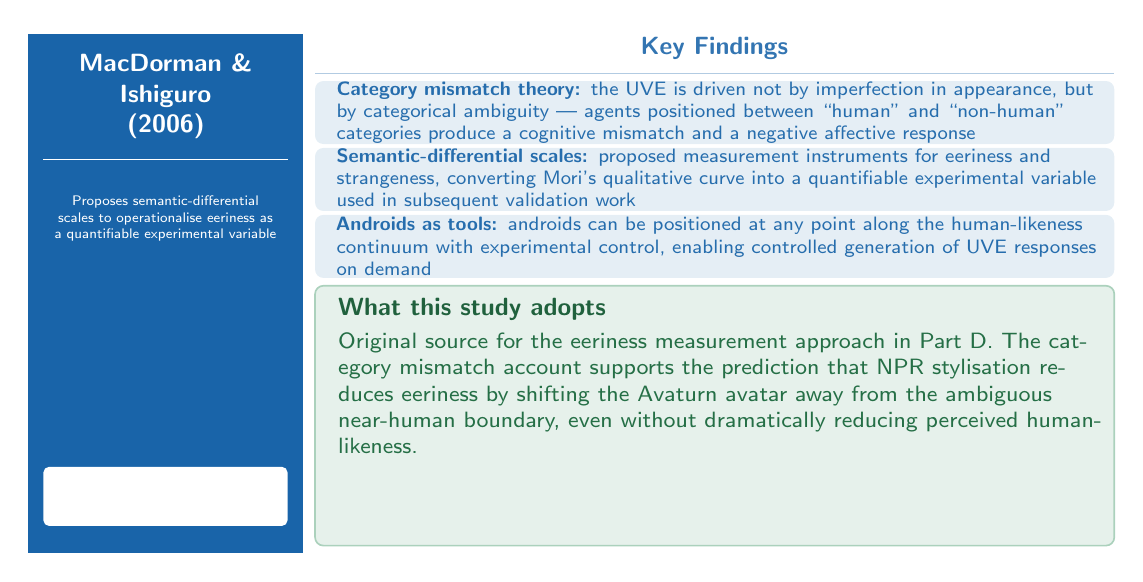
\begin{tikzpicture}[x=1cm, y=1cm]
\fill[kblue!90] (0.0,0.0) rectangle (3.5,6.6);
\node[font=\small\sffamily\bfseries, text=white, align=center, text width=3.1cm]
  at (1.75,5.80) {MacDorman \&\\Ishiguro\\(2006)};
\draw[white!30, line width=0.3pt] (0.2,5.00) -- (3.3,5.00);
\node[font=\tiny\sffamily, text=white!85, align=center, text width=3.0cm]
  at (1.75,4.25) {Proposes semantic-differential scales to operationalise eeriness as a quantifiable experimental variable};
\fill[white!20, rounded corners=2pt] (0.2,0.35) rectangle (3.3,1.10);
\node[font=\tiny\sffamily\bfseries, text=white, align=center]
  at (1.75,0.72) {Theoretical\\pilot, no full stats};
\node[font=\small\sffamily\bfseries\color{kblue!80}] at (8.72,6.42) {Key Findings};
\draw[kblue!30, line width=0.3pt] (3.65,6.10) -- (13.8,6.10);
\fill[kblue!10, rounded corners=3pt] (3.65,5.20) rectangle (13.8,6.00);
\node[font=\scriptsize\sffamily\color{kblue!85}, anchor=west, text width=9.65cm]
  at (3.80,5.60) {\textbf{Category mismatch theory:} the UVE is driven not by imperfection in appearance, but by categorical ambiguity --- agents positioned between ``human'' and ``non-human'' categories produce a cognitive mismatch and a negative affective response};
\fill[kblue!10, rounded corners=3pt] (3.65,4.35) rectangle (13.8,5.15);
\node[font=\scriptsize\sffamily\color{kblue!85}, anchor=west, text width=9.65cm]
  at (3.80,4.75) {\textbf{Semantic-differential scales:} proposed measurement instruments for eeriness and strangeness, converting Mori's qualitative curve into a quantifiable experimental variable used in subsequent validation work};
\fill[kblue!10, rounded corners=3pt] (3.65,3.50) rectangle (13.8,4.30);
\node[font=\scriptsize\sffamily\color{kblue!85}, anchor=west, text width=9.65cm]
  at (3.80,3.90) {\textbf{Androids as tools:} androids can be positioned at any point along the human-likeness continuum with experimental control, enabling controlled generation of UVE responses on demand};
\fill[kgreen!12, draw=kgreen!40, rounded corners=3pt, line width=0.6pt]
  (3.65,0.1) rectangle (13.8,3.40);
\node[font=\small\sffamily\bfseries\color{kgreen!70!black}, anchor=west]
  at (3.82,3.1) {What this study adopts};
\node[font=\footnotesize\sffamily\color{kgreen!80!black}, anchor=north west, text width=9.65cm]
  at (3.82,2.92) {Original source for the eeriness measurement approach in Part D. The category mismatch account supports the prediction that NPR stylisation reduces eeriness by shifting the Avaturn avatar away from the ambiguous near-human boundary, even without dramatically reducing perceived human-likeness.};
\end{tikzpicture}
\end{center}
\end{frame}

%% ═══════════════════════════════════════════════════════════════════════════
%% Ho & MacDorman 2010
%% ═══════════════════════════════════════════════════════════════════════════
\begin{frame}{Ho \& MacDorman (2010) \textnormal{\normalsize --- Eeriness Scale}}
\begin{center}
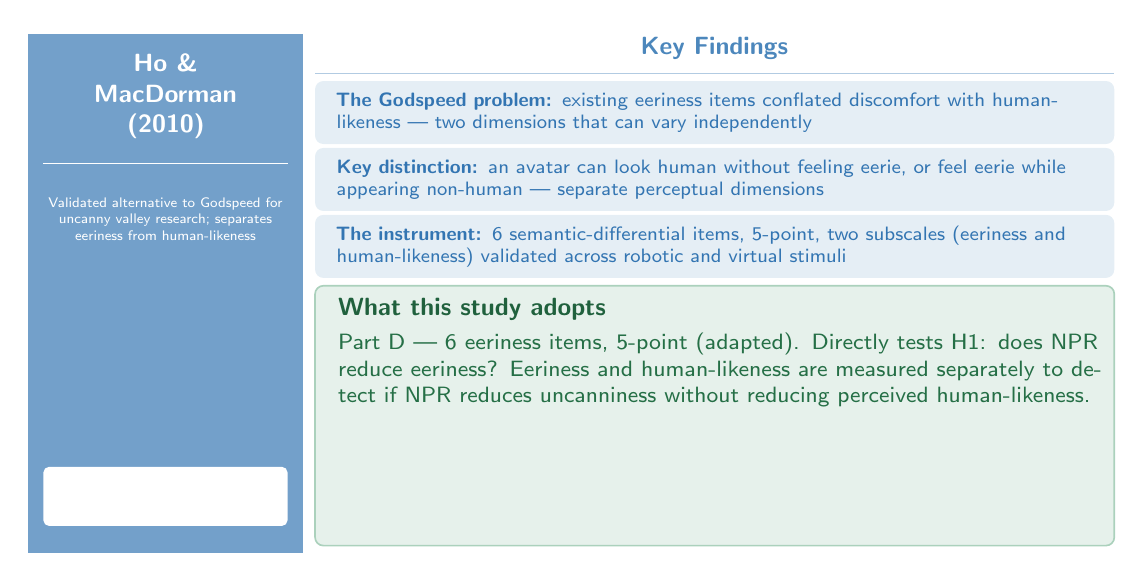
\begin{tikzpicture}[x=1cm, y=1cm]
\fill[kblue!55] (0.0,0.0) rectangle (3.5,6.6);
\node[font=\small\sffamily\bfseries, text=white, align=center, text width=3.1cm]
  at (1.75,5.8) {Ho \&\\MacDorman\\(2010)};
\draw[white!30, line width=0.3pt] (0.2,4.95) -- (3.3,4.95);
\node[font=\tiny\sffamily, text=white!85, align=center, text width=3.0cm]
  at (1.75,4.25) {Validated alternative to Godspeed for uncanny valley research; separates eeriness from human-likeness};
\fill[white!20, rounded corners=2pt] (0.2,0.35) rectangle (3.3,1.10);
\node[font=\tiny\sffamily\bfseries, text=white, align=center]
  at (1.75,0.72) {Validation study\\multiple stimulus types};
\node[font=\small\sffamily\bfseries\color{kblue!70}] at (8.72,6.42) {Key Findings};
\draw[kblue!30, line width=0.3pt] (3.65,6.10) -- (13.8,6.10);
\fill[kblue!10, rounded corners=3pt] (3.65,5.20) rectangle (13.8,6.00);
\node[font=\scriptsize\sffamily\color{kblue!80}, anchor=west, text width=9.65cm]
  at (3.80,5.60) {\textbf{The Godspeed problem:} existing eeriness items conflated discomfort with human-likeness --- two dimensions that can vary independently};
\fill[kblue!10, rounded corners=3pt] (3.65,4.35) rectangle (13.8,5.15);
\node[font=\scriptsize\sffamily\color{kblue!80}, anchor=west, text width=9.65cm]
  at (3.80,4.75) {\textbf{Key distinction:} an avatar can look human without feeling eerie, or feel eerie while appearing non-human --- separate perceptual dimensions};
\fill[kblue!10, rounded corners=3pt] (3.65,3.50) rectangle (13.8,4.30);
\node[font=\scriptsize\sffamily\color{kblue!80}, anchor=west, text width=9.65cm]
  at (3.80,3.90) {\textbf{The instrument:} 6 semantic-differential items, 5-point, two subscales (eeriness and human-likeness) validated across robotic and virtual stimuli};
\fill[kgreen!12, draw=kgreen!40, rounded corners=3pt, line width=0.6pt]
  (3.65,0.1) rectangle (13.8,3.40);
\node[font=\small\sffamily\bfseries\color{kgreen!70!black}, anchor=west]
  at (3.82,3.1) {What this study adopts};
\node[font=\footnotesize\sffamily\color{kgreen!80!black}, anchor=north west, text width=9.65cm]
  at (3.82,2.92) {Part D --- 6 eeriness items, 5-point (adapted). Directly tests H1: does NPR reduce eeriness? Eeriness and human-likeness are measured separately to detect if NPR reduces uncanniness without reducing perceived human-likeness.};
\end{tikzpicture}
\end{center}
\end{frame}

%% ═══════════════════════════════════════════════════════════════════════════
%% McDonnell et al. 2012
%% ═══════════════════════════════════════════════════════════════════════════
\begin{frame}{McDonnell et al. (2012) \textnormal{\normalsize --- Render Me Real?}}
\begin{center}
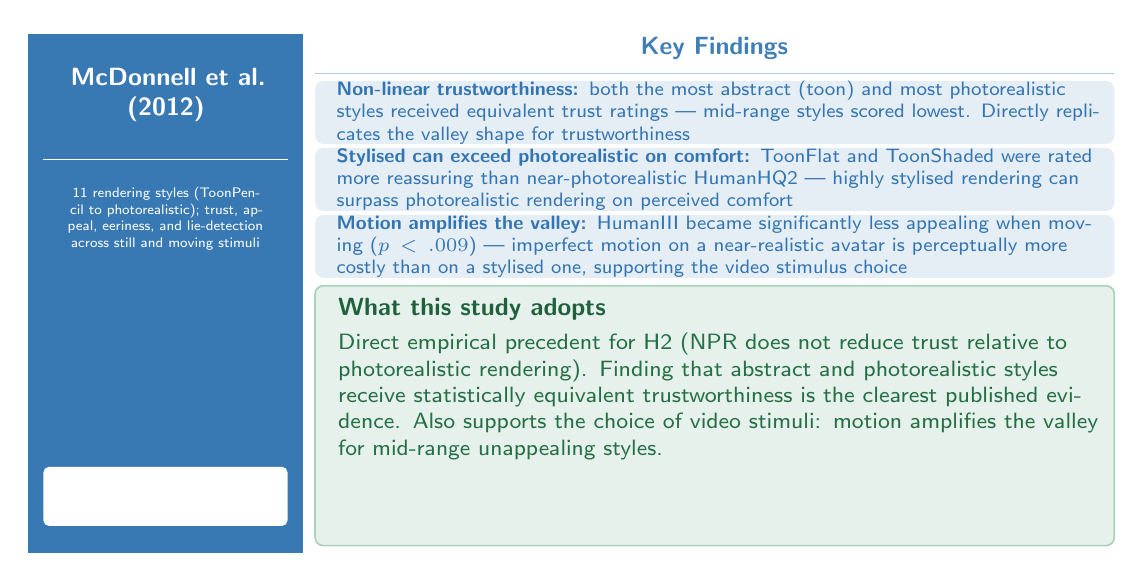
\begin{tikzpicture}[x=1cm, y=1cm]
\fill[kblue!78] (0.0,0.0) rectangle (3.5,6.6);
\node[font=\small\sffamily\bfseries, text=white, align=center, text width=3.1cm]
  at (1.75,5.82) {McDonnell et al.\\(2012)};
\draw[white!30, line width=0.3pt] (0.2,5.00) -- (3.3,5.00);
\node[font=\tiny\sffamily, text=white!85, align=center, text width=3.0cm]
  at (1.75,4.25) {11 rendering styles (ToonPencil to photorealistic); trust, appeal, eeriness, and lie-detection across still and moving stimuli};
\fill[white!20, rounded corners=2pt] (0.2,0.35) rectangle (3.3,1.10);
\node[font=\tiny\sffamily\bfseries, text=white, align=center]
  at (1.75,0.72) {Empirical\\3 experiments};
\node[font=\small\sffamily\bfseries\color{kblue!75}] at (8.72,6.42) {Key Findings};
\draw[kblue!30, line width=0.3pt] (3.65,6.10) -- (13.8,6.10);
\fill[kblue!10, rounded corners=3pt] (3.65,5.20) rectangle (13.8,6.00);
\node[font=\scriptsize\sffamily\color{kblue!80}, anchor=west, text width=9.65cm]
  at (3.80,5.60) {\textbf{Non-linear trustworthiness:} both the most abstract (toon) and most photorealistic styles received equivalent trust ratings --- mid-range styles scored lowest. Directly replicates the valley shape for trustworthiness};
\fill[kblue!10, rounded corners=3pt] (3.65,4.35) rectangle (13.8,5.15);
\node[font=\scriptsize\sffamily\color{kblue!80}, anchor=west, text width=9.65cm]
  at (3.80,4.75) {\textbf{Stylised can exceed photorealistic on comfort:} ToonFlat and ToonShaded were rated more reassuring than near-photorealistic HumanHQ2 --- highly stylised rendering can surpass photorealistic rendering on perceived comfort};
\fill[kblue!10, rounded corners=3pt] (3.65,3.50) rectangle (13.8,4.30);
\node[font=\scriptsize\sffamily\color{kblue!80}, anchor=west, text width=9.65cm]
  at (3.80,3.90) {\textbf{Motion amplifies the valley:} HumanIII became significantly less appealing when moving ($p < .009$) --- imperfect motion on a near-realistic avatar is perceptually more costly than on a stylised one, supporting the video stimulus choice};
\fill[kgreen!12, draw=kgreen!40, rounded corners=3pt, line width=0.6pt]
  (3.65,0.1) rectangle (13.8,3.40);
\node[font=\small\sffamily\bfseries\color{kgreen!70!black}, anchor=west]
  at (3.82,3.1) {What this study adopts};
\node[font=\footnotesize\sffamily\color{kgreen!80!black}, anchor=north west, text width=9.65cm]
  at (3.82,2.92) {Direct empirical precedent for H2 (NPR does not reduce trust relative to photorealistic rendering). Finding that abstract and photorealistic styles receive statistically equivalent trustworthiness is the clearest published evidence. Also supports the choice of video stimuli: motion amplifies the valley for mid-range unappealing styles.};
\end{tikzpicture}
\end{center}
\end{frame}

%% ═══════════════════════════════════════════════════════════════════════════
%% Seymour et al. 2021
%% ═══════════════════════════════════════════════════════════════════════════
\begin{frame}{Seymour et al. (2021) \textnormal{\normalsize --- Have We Crossed the Uncanny Valley?}}
\begin{center}
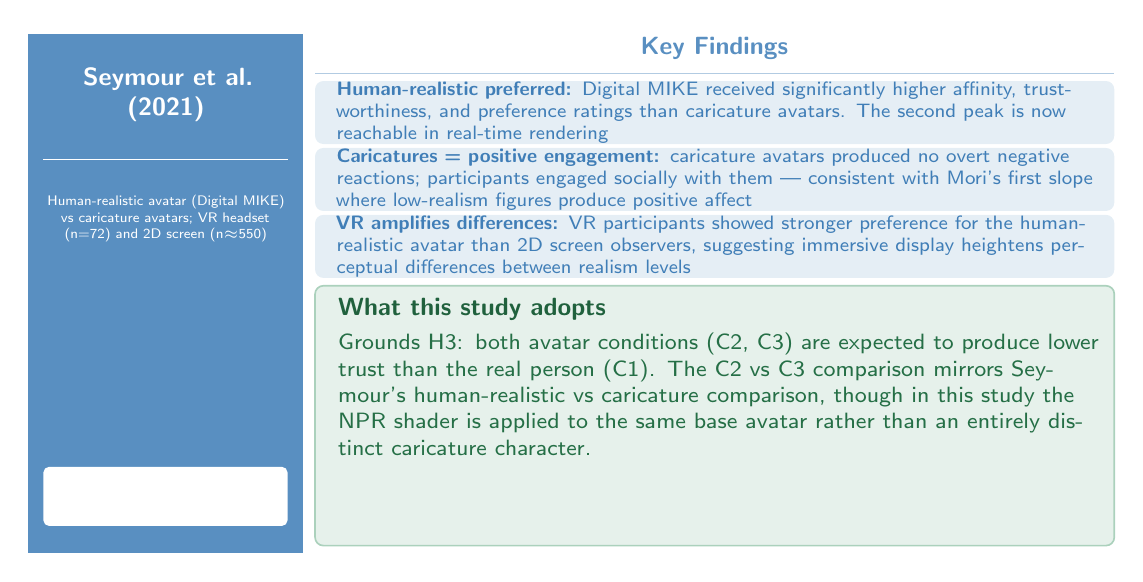
\begin{tikzpicture}[x=1cm, y=1cm]
\fill[kblue!65] (0.0,0.0) rectangle (3.5,6.6);
\node[font=\small\sffamily\bfseries, text=white, align=center, text width=3.1cm]
  at (1.75,5.82) {Seymour et al.\\(2021)};
\draw[white!30, line width=0.3pt] (0.2,5.00) -- (3.3,5.00);
\node[font=\tiny\sffamily, text=white!85, align=center, text width=3.0cm]
  at (1.75,4.25) {Human-realistic avatar (Digital MIKE) vs caricature avatars; VR headset (n=72) and 2D screen (n$\approx$550)};
\fill[white!20, rounded corners=2pt] (0.2,0.35) rectangle (3.3,1.10);
\node[font=\tiny\sffamily\bfseries, text=white, align=center]
  at (1.75,0.72) {Empirical\\n $\approx$ 622};
\node[font=\small\sffamily\bfseries\color{kblue!65}] at (8.72,6.42) {Key Findings};
\draw[kblue!30, line width=0.3pt] (3.65,6.10) -- (13.8,6.10);
\fill[kblue!10, rounded corners=3pt] (3.65,5.20) rectangle (13.8,6.00);
\node[font=\scriptsize\sffamily\color{kblue!75}, anchor=west, text width=9.65cm]
  at (3.80,5.60) {\textbf{Human-realistic preferred:} Digital MIKE received significantly higher affinity, trustworthiness, and preference ratings than caricature avatars. The second peak is now reachable in real-time rendering};
\fill[kblue!10, rounded corners=3pt] (3.65,4.35) rectangle (13.8,5.15);
\node[font=\scriptsize\sffamily\color{kblue!75}, anchor=west, text width=9.65cm]
  at (3.80,4.75) {\textbf{Caricatures = positive engagement:} caricature avatars produced no overt negative reactions; participants engaged socially with them --- consistent with Mori's first slope where low-realism figures produce positive affect};
\fill[kblue!10, rounded corners=3pt] (3.65,3.50) rectangle (13.8,4.30);
\node[font=\scriptsize\sffamily\color{kblue!75}, anchor=west, text width=9.65cm]
  at (3.80,3.90) {\textbf{VR amplifies differences:} VR participants showed stronger preference for the human-realistic avatar than 2D screen observers, suggesting immersive display heightens perceptual differences between realism levels};
\fill[kgreen!12, draw=kgreen!40, rounded corners=3pt, line width=0.6pt]
  (3.65,0.1) rectangle (13.8,3.40);
\node[font=\small\sffamily\bfseries\color{kgreen!70!black}, anchor=west]
  at (3.82,3.1) {What this study adopts};
\node[font=\footnotesize\sffamily\color{kgreen!80!black}, anchor=north west, text width=9.65cm]
  at (3.82,2.92) {Grounds H3: both avatar conditions (C2, C3) are expected to produce lower trust than the real person (C1). The C2 vs C3 comparison mirrors Seymour's human-realistic vs caricature comparison, though in this study the NPR shader is applied to the same base avatar rather than an entirely distinct caricature character.};
\end{tikzpicture}
\end{center}
\end{frame}

\end{document}
